\section{Experiments}
\label{sec:Experiments}

To evaluate the performance of PSE, we implemented a prototype in C++ that employs ExactMC as the model counter.
We evaluate PSE in 361 benchmarks, including the QIF  benchmarks~\cite{fremont2017maximum}, combinatorial circuits, plan recognition~\cite{soos2020tinted}, bit-blasted versions of SMTLIB benchmarks~\cite{sharma2019ganak}, and QBFEval competitions~\cite{golia2022scalable}. %~\cite{qbfeval2017, qbfeval2018}. 
All experiments were run on a computer with Intel(R) Core(TM) i9-10920X CPU @ 3.50GHz and 32GB RAM.
RAM. 
Each instance was run on a single core with a timeout
of 3000 seconds and 8GB memory.


Through our evaluations and analysis, we sought to answer the following research questions:
\begin{itemize}
	\item \textbf{RQ1:} How does the runtime performance of PSE compare to the state-of-the-art precise Shannon entropy tools?
	\item \textbf{RQ2:} How does the runtime performance of PSE compare to the state-of-the-art Shannon entropy estimation tool?
	\item \textbf{RQ2:} How do the utilized methods impact the runtime performance of PSE? 
\end{itemize}


\subsection{Comparison with precise Shannon entropy tools}

\begin{table}[h!]
	\centering
	\resizebox{\linewidth}{!}
	{
		\begin{tabular}{ cccccccccc } 
			\toprule 
			\multirow{2}*{instance} & \multirow{2}*{$\left| X \right|$} & \multirow{2}*{$\left| Y \right|$} & \multicolumn{2}{c}{baseline-SharpSAT-TD} & \multicolumn{2}{c}{baseline-ExactMC} & \multicolumn{2}{c}{PSE} \\
			
			\cmidrule(r){4-5}   
			\cmidrule(r){6-7}
			\cmidrule(r){8-9}  
			
			& & & Entropy & Time(s) & Entropy & Time(s) & Entropy & Time(s)\\ 
			
			\midrule  
			blasted$\_$case102.cnf & 11 & 23 & 8 & 81.29 & 8 & 0.39 & 8 & 0.16 \\
			s27$\_$15$\_$7.cnf & 7 & 25 & 3.3 & 142.77  & 3.3 & 0.15 & 3.3 & 0.14 \\
			small-bug1-fixpoint-5.cnf & 66 & 21 & 12.81 & 79.51 & 12.81 & 2.99 & 12.81 & 0.18 \\
			small-bug1-fixpoint-6.cnf & 79 & 25 & 15.31 & 1406.47 & 15.31 & 51.9 & 15.31 & 0.21 \\
			blasted$\_$case144.cnf & 138 & 627 & - & - & - & - & 77.62 & 35.42 \\
			s1423a$\_$15$\_$7.cnf & 91 & 773 & - & - & - & - &  88.17 & 232.65 \\
			s382$\_$15$\_$7.cnf & 24 & 326 & - & - & - & - & 23.58 & 0.22 \\
			CVE-2007-2875.cnf & 752 & 32 & - & - & - & - & 32 & 0.72 \\
			10.sk$\_$1$\_$46.cnf & 47 & 1447 & - & - & - & - & 13.58 & 0.18 \\
			
			\bottomrule
		\end{tabular}
	}
	\caption{Entropy computing performance of baseline and PSE. "-" represents that the entropy cannot be solved within the specified time limit.
	\label{table:1}
	}
\end{table}
The existing precise Shannon entropy tools do not use the techniques in the state-of-the-art model counters.
Just like~\cite{golia2022scalable}, we implemented the precise Shannon entropy baseline with state-of-the-art model counting techniques.
In the baseline, we enumerate each assignment $\sigma \in \mathit{Sol}(\varphi)_{\downarrow Y}$ and compute $p_{\sigma} = \frac{\left| \mathit{Sol}(\varphi(Y \mapsto \sigma)) \right|}{ \left| \mathit{Sol}(\varphi)_{\downarrow X} \right| }$, where $\mathit{Sol}(\varphi(Y \mapsto \sigma))$ denotes the set of solutions of $\varphi(Y \mapsto \sigma)$ and $\mathit{Sol}(\varphi)_{\downarrow X}$ denotes the set of solutions of $\varphi$ projected to $X$.
As can be seen from the previous proposition, $| \mathit{Sol}(\varphi)_{\downarrow X} |$ can be replaced by $| \mathit{Sol}(\varphi) |$.
Finally, entropy is computed as $H(\varphi) = \sum_{\sigma \in 2^Y} -p_{\sigma} \log {p_{\sigma}} $.
For a formula with an output set size of $m$, $2^m$ model counting queries are required, and we chose the state-of-the-art model counters SharpSAT-TD and ExactMC to the model counting queries, respectively.

In our experiment, the baseline with SharpSAT-TD (resp. ExactMC) can only solve 17 instances within the specified time of 3000 seconds, while PSE can solve 289 instances. 
Table \ref{table:1} shows the comparison between baseline and PSE on some instances.
The results show a significant improvement in the efficiency of PSE for computing the precise Shannon entropy, which answers \textbf{RQ1} as well.


\begin{comment}
	\begin{table}[h!]
		\centering
		\begin{tabular}{ cccc } 
			\toprule 
			domains & $\#$ instances & PSE & EntropyEstimation 
			\\ 
			\midrule 
			BlastedSMT & 217 & \textbf{174} & 160 \\ 
			
			Circuit & 91 & \textbf{70} & 64 \\
			
			Verification & 27 & \textbf{27} & 14 \\ 
			
			QIF & 3 & \textbf{3} & \textbf{3} \\ 
			
			QBF & 23 & 15 & \textbf{23} \\ 
			
			Toal & 361 & \textbf{290} & 265 \\
			\bottomrule
		\end{tabular}
		\caption{Comparative entropy counting performance between PSE and EntropyEstimation, where each cell below tool refers to the number of solved instances.}
		\label{table:2}
	\end{table}
\end{comment}


%\subsection{Comparison with EntropyEstimation}
\subsection{Comparison with Shannon entropy estimation tool}
We compare PSE with EntropyEstimation, the current state-of-the-art Shannon entropy estimation tool on 361 instances. 
Table \ref{table:2} shows the performance of PSE and EntropyEstimation~\cite{golia2022scalable} in entropy computing.


\begin{table}[h!]
	\centering
	\begin{tabular}{ ccccc } 
		\toprule 
		\multirow{2}{*}{tool}  & \multicolumn{3}{c}{Instances Solved} & \multirow{2}{*}{Average PAR-2 score} \\
		 \cline{2-4}
		& Unique & Fastest & Total \\ 
		\midrule 
		EntropyEstimation & 10 & 0 & 264 & 1574.59 \\ 
		
		PSE & \textbf{35} & \textbf{254} & \textbf{289} & \textbf{1193.37} \\
		\bottomrule
	\end{tabular}
	\caption{Detailed performance comparison of PSE and EntropyEstimation. Unique represents the number of instances that can only be solved by a specific tool. Fastest represents the number of instances that a tool solves with the shortest time.}
	\label{table:2}
\end{table}

\begin{figure}[htbp]
	\centering
	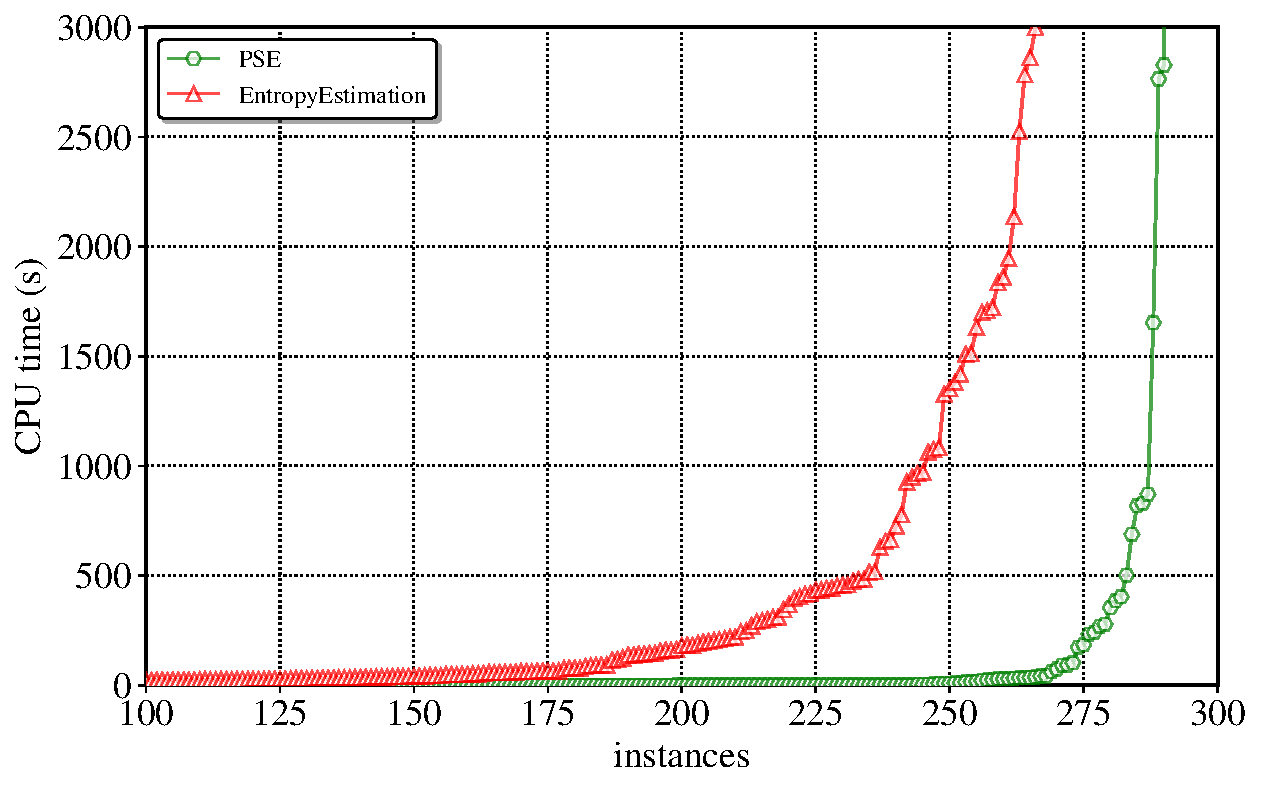
\includegraphics[width=7cm,height=8cm]{figures/PSEvsEntropyEstimation.pdf}
	\caption{Cactus plot comparing the computing time of PSE and EntropyEstimation.
	}
	\label{figure:2}
\end{figure} 

From Table \ref{table:2}, it can be seen that out of a total of 361 instances, under the time limit of 3000 seconds, our tool PSE is able to solve 25 more instances than EntropyEstimation, and the overall performance is better. 
For all instances where both PSE and EntropyEstimation can be solved, PSE has a shorter computing time, as well as a much smaller average PAR-2 score~\footnote{The average PAR-2 scoring scheme gives a penalized average runtime, assigning a runtime of two times the time limit for each benchmark that the tool fails to solve} than EntropyEstimation.
Figure \ref{figure:2} shows the cactus plot of runtime for PSE and EntropyEstimation, where the $x$-axis represents the number of benchmarks and the $y$-axis represents the runtime.

%It can be concluded that PSE is significantly more efficient than EntropyEstimation in computing the same instances that can be solved by both PSE and EntropyEstimation.
Meanwhile, we also observed that there were some instances that PSE could not solve while EntropyEstimation could.
We observed in our experiments that in the instances where PSE could not be solved, the number of model counting queries was so high that it had reached an order of magnitude of ten million and still did not solve for entropy.
We believe this may have reached the bottleneck of precise Shannon entropy computing.
Therefore, we believe that more powerful techniques are needed to accurately solve the entropy of these instances.
We analyze that better preprocessing methods and more suitable variable heuristics for entropy computing may become a breakthrough.
However, we need to emphasize that EntropyEstimation is only a Shannon entropy estimation tool, and the entropy it obtains is subject to a certain degree of error. 
Our precise Shannon entropy tool PSE performs better than entropy estimators in most instances, which demonstrates that our techniques significantly enhance the scalability of precise Shannon entropy.
%From the results, we can more intuitively observe that in the majority of instances, the performance of PSE is significantly better than EntropyEstimation which provides an affirmative answer to \textbf{RQ2}.
Based on the results, it is evident that PSE outperforms EntropyEstimation in the majority of instances. This provides a positive answer to \textbf{RQ2}.

%These experimental results show that PSE has significant advantages over both state-of-the-art precise and approximate entropy tools.
%This also provides an affirmative answer to \textbf{RQ1}.


\subsection{Impact of algorithmic configurations}
To better verify the effectiveness of the PSE methods and answer \textbf{RQ3}, we conducted a comparative study on all the utilized methods, including methods for the $Y$-stage: \textbf{Implied Literal}, \textbf{YCache}, \textbf{Pre}, variable decision heuristics(\textbf{minfill}, \textbf{DLCP}, \textbf{SharpSAT-TD heuristic}, \textbf{VSADS}), and methods for the $X$-stage: \textbf{XCache} and \textbf{ConditionedCounting}.
According to the principle of control variables, we designed ablation experiments to verify the effectiveness of each method, and each experiment was only different from the tool PSE in one method.
The cactus plot for the different methods is shown in Figure \ref{figure:3}, where PSE represents our tool, PSE-wo-Pre means that \textbf{Pre} is turned off in PSE.
PSE-ConditionedCounting indicates that PSE employed the \textbf{ConditionedCounting} method rather than \textbf{SharedCounting} in the $X$-stage.
PSE-wo-XCache indicates that the caching method is turned off in PSE in the $X$-stage. 
PSE-wo-YCache indicates that the caching method is turned off in PSE in the $Y$-stage.
PSE-wo-ImpliedLiteral indicates that PSE does not employ the \textbf{Implied Literal} in the $Y$-stage.
PSE-dynamic-SharpSAT-TD means that PSE replaces the \textbf{minfill} static variable order with the dynamic variable order: the variable decision-making heuristic method of SharpSAT-TD (all other configurations are the same as in PSE, only the variable decision-making heuristic is different).
Similarly, PSE-dynamic-DLCP and PSE-dynamic-VSADS respectively indicate the selection of dynamic heuristic \textbf{DLCP} and \textbf{VSADS}.

As can be seen from the experimental results, the power of implied literal is very strong. 
The effect of caching is also significant, as has been demonstrated in previous studies of knowledge compilation.
Although the effect of preprocessing is not very significant, it can still increase the number of instances solved.
The heuristic strategies minfill and SharpSAT-TD heuristic both performed well, and the results indicate that the static heuristic minfill is more suitable for entropy computing.
In the technique of the $X$-stage, the \textbf{ConditionedCounting} method performs better than \textbf{SharedCounting} without \textbf{XCache}, but not as well as the \textbf{SharedCounting} method.
This comparative experiment indicates that the shared component caching is quite effective.
The biggest advantage of the \textbf{ConditionedCounting} method is that its time complexity is linear~\cite{lai2017new}, although it also has a major disadvantage in that we need to construct an ADD-L based on the static variable order first, which is a process with a large time overhead for more complex problems.
Although the \textbf{ConditionedCounting} method is not the most effective, we believe it is still a promising and scalable method. 
For instances where an ADD-L can be constructed quickly based on the static variable order, the \textbf{ConditionedCounting} method may work better than the SharedCounting method when it is difficult to model counting in $X$-stage. 
The \textbf{ConditionedCounting} method is not the best method, but we believe it is still a promising and scalable method.
Finally, PSE selects the \textbf{SharedCounting} strategy in the $X$-stage, and chooses \textbf{YCache}, \textbf{Implied Literal}, \textbf{Pre}, and the \textbf{minfill} heuristic method in the $Y$-stage.
	
\begin{figure}[htbp]
	\centering
	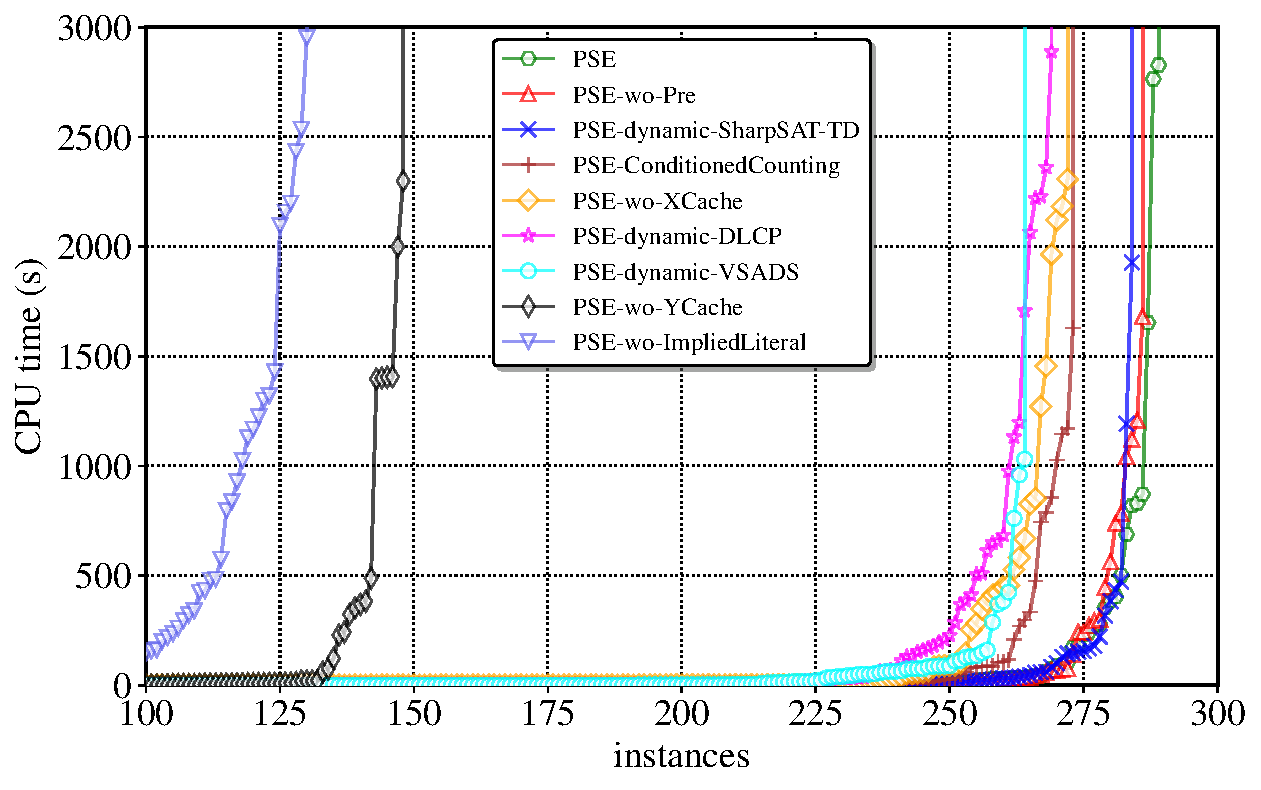
\includegraphics[width=12cm,height=8cm]{figures/Configuration_compare.pdf}
	\caption{Cactus plot comparing different methods.}
	\label{figure:3}
\end{figure} 


\begin{comment}
	\subsection{Impact of pre-process}
	We compare the effects of the preprocessing techniques mentioned in Section 4 on PSE.
	We use the term "Pre" to refer to the preprocessing in ExactMC. "Pre + Liteq" means preprocessing plus literal equivalence strategy. "Pre + Liteq\_New" refers to preprocessing plus the improved literal equivalence strategy proposed in this paper.
	Figure \ref{figure:3} shows the cactus plot comparing three different preprocessing strategies, where the x-axis represents the number of solved instances and the y-axis represents the running time.
	In order to visualise the efficiency gap between different preprocessing methods more intuitively, we removed 250 instances that could be solved by PSE within 1s.
	From the results, it is clear that the literal equivalence strategy is an enhancement to entropy computing and Liteq\_New performs the best. 
	Using literal equivalence strategy can reduce the average PAR-2 score from 1287.38 to 1257.83. while Liteq\_New strategy can make the average PAR-2 score reduced to 1193.37.
	
	
	
	
	\begin{figure}[htbp]
		\centering
		\includegraphics[width=12cm,height=8cm]{figures/Preprocess.pdf}
		\caption{Cactus plot comparing different preprocessing strategies.
		}
		\label{figure:3}
	\end{figure} 
\end{comment}

